\documentclass[a4paper,12pt]{article} % тип документа

% Поля страниц
\usepackage[left=2.5cm,right=2.5cm,
top=2cm,bottom=2cm,bindingoffset=0cm]{geometry}

%Пакет дял таблиц   
\usepackage{multirow}
\usepackage{longtable}

%Отступ после заголовка    
\usepackage{indentfirst}


% Рисунки
\usepackage{floatrow,graphicx,calc}
\usepackage{wrapfig}

% Создаёем новый разделитель
\DeclareFloatSeparators{mysep}{\hspace{1cm}}

% Ссылки?
\usepackage{hyperref}
\usepackage[rgb]{xcolor}
\hypersetup{				% Гиперссылки
	colorlinks=true,       	% false: ссылки в рамках
	urlcolor=blue          % на URL
}


%  Русский язык
\usepackage[T2A]{fontenc}			% кодировка
\usepackage[utf8]{inputenc}			% кодировка исходного текста
\usepackage[english,russian]{babel}	% локализация и переносы


% Математика
\usepackage{amsmath,amsfonts,amssymb,amsthm,mathtools, mathrsfs}


% Что-то 
\usepackage{wasysym}


\begin{document}
	\begin{center}
		\footnotesize{ФЕДЕРАЛЬНОЕ ГОСУДАРСТВЕННОЕ АВТОНОМНОЕ ОБРАЗОВАТЕЛЬНОЕ 			УЧРЕЖДЕНИЕ ВЫСШЕГО ОБРАЗОВАНИЯ}\\
		\footnotesize{МОСКОВСКИЙ ФИЗИКО-ТЕХНИЧЕСКИЙ ИНСТИТУТ\\(НАЦИОНАЛЬНЫЙ 			ИССЛЕДОВАТЕЛЬСКИЙ УНИВЕРСИТЕТ)}\\
		\footnotesize{ФАКУЛЬТЕТ ОБЩЕЙ И ПРИКЛАДНОЙ ФИЗИКИ\\}
		\hfill \break
		\hfill\break
		\hfill\break
		\hfill \break
		\hfill \break
		\hfill \break
		\hfill \break
		\hfill \break
		\hfill \break
		\hfill \break
		\hfill \break
		\hfill \break
		\hfill \break
		\hfill \break
		\large{Лабораторная работа № 3.2.5\\\textbf{Вынужденные колебания в электрическом контуре}}\\
		\hfill \break
		\hfill \break
		\hfill \break
		\begin{flushright}
			Серебренников Даниил\\
			Группа Б02-826
		\end{flushright}
		\hfill \break
		\hfill \break
		\hfill \break
		\hfill \break
		\hfill \break
	\end{center}
	\hfill \break
	\hfill \break
	\hfill \break
	\hfill \break
	\hfill \break
	\hfill \break
	\begin{center}
		Долгопрудный, 2019 г.
	\end{center}
	\thispagestyle{empty}
	\newpage
	
	\textbf{Цель работы:} исследование вынужденных колебаний и процессов их установления.
	
	\textbf{В работе используются:} генератор звуковой частоты, осциллограф, вольтметр, частотометр, ёмкость, индуктивность, магазин сопротивлений, универслаьный мост.
	
	
\section{Теоретическая часть}
	При подключении к контуру внешнего источника в нём возникают колебания, которые можно представить как суперпозицию двух синусоид: первая -- с частотой собственных колебаний контура $\omega$ и амплитудой, экспоненциально убывающей со временем; вторая -- с частотой внешнего источника $\Omega$ и постоянной амплитудой. Со временем собственные колебания затухают, и в контуре устанавливаются вынужденные колебания. Амплитуда этих колебаний максимальна при совпадении частоты $\Omega$ внешнего сигнала с собственной частотой контура $\omega_0$. Это явление называют резонансом. Зависимость амплитуды установившихся колебаний от частоты внешнего напряжения носит названия резонансной кривой.	

\section{Экспериментальная установка}
	Схема установки для исследования вынужденных колебаний приведена на рис.~\ref{ris:ustanovka}. Колебательный контур состоит из ёмкости $C = 0,1$ мкФ, индуктивности $L = 100$ мГн и переменного сопроьтивления $R$.	
	\begin{figure}[H]
		\center{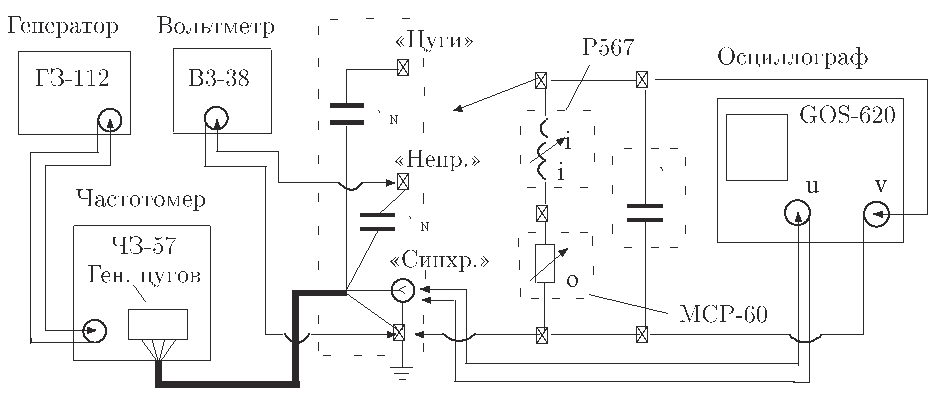
\includegraphics[scale=1]{ustanovka.pdf}}
		\caption{Схема экспериментальной установки для исследования вынужденных колебаний.}
		\label{ris:ustanovka}
	\end{figure}

\newpage
\section{Экспериментальные данные}
	\floatsetup[table]{capposition=top}	
	\begin{table}[H]
		\caption{Параметры установки.}
		\label{table:const}
		\begin{tabular}{|c|c|c|c|c|c|}
			\hline
			& $U_0$, мВ & $\nu_0$, Гц           & $L$, мГн                & $C$, мкФ             & $R_L$, Ом              \\ \hline
			$R = 0$ Ом   & 100       & \multirow{2}{*}{1567} & \multirow{2}{*}{100,01} & \multirow{2}{*}{0,1} & \multirow{2}{*}{25,58} \\ \cline{1-2}
			$R = 100$ Ом & 10        &                       &                         &                      &                        \\ \hline
		\end{tabular}
	\end{table}

		\floatsetup[table]{capposition=top}	
		\begin{table}[H]
			\caption{Экспериментальные данные.}
			\label{table:experiment}
			\begin{tabular}{|c|c|c|c|}
				\hline
				\multicolumn{2}{|c|}{$R = 0$ Ом} & \multicolumn{2}{c|}{$R = 100$ Ом} \\ \hline
				$\nu/\nu_0$       & $U/U_0$      & $\nu/\nu_0$       & $U/U_0$       \\ \hline
				1,00              & 1,00         & 1,004             & 1             \\ \hline
				1,01              & 0,90         & 1,041             & 0,9           \\ \hline
				1,01              & 0,80         & 1,062             & 0,8           \\ \hline
				1,01              & 0,70         & 1,084             & 0,7           \\ \hline
				1,02              & 0,60         & 1,115             & 0,6           \\ \hline
				1,02              & 0,50         & 1,158             & 0,5           \\ \hline
				1,03              & 0,40         & 1,236             & 0,4           \\ \hline
				1,05              & 0,30         & 1,410             & 0,3           \\ \hline
				1,00              & 1,00         & 1,031             & 0,94          \\ \hline
				0,99              & 0,90         & 1,049             & 0,86          \\ \hline
				0,99              & 0,80         & 1,026             & 0,96          \\ \hline
				0,99              & 0,70         & 1,013             & 1             \\ \hline
				0,98              & 0,60         & 0,979             & 0,9           \\ \hline
				0,98              & 0,50         & 0,966             & 0,8           \\ \hline
				0,97              & 0,40         & 0,951             & 0,7           \\ \hline
				0,96              & 0,30         & 0,936             & 0,6           \\ \hline
				&              & 0,921             & 0,5           \\ \hline
				&              & 0,899             & 0,4           \\ \hline
				&              & 0,869             & 0,3           \\ \hline
				&              & 0,992             & 0,96          \\ \hline
				&              & 0,987             & 0,94          \\ \hline
				&              & 0,973             & 0,86          \\ \hline
			\end{tabular}
		\end{table}
		
		
	\floatsetup[table]{capposition=top}	
	\begin{table}[H]
		\caption{Добротность.}
		\label{table:dobrotnost}
		\begin{tabular}{|c||c|c|c|c|}
			\hline
			\multirow{2}{*}{$R$, Ом}  & \multicolumn{4}{c|}{$Q$} \\ \cline{2-5}
			& $\omega_0/\Omega$ & нараст & убыв & $f(LCR)$ \\
			\hline \hline
			0  & $38,9 \pm 1,5$  & --- & $34,5 \pm 5,4$ & $39,1 \pm 0,8$ \\
			100  & $7,7 \pm 0,6$ & $7,9 \pm 0,9$ & $8,03 \pm 0,6$ & $7,96 \pm 0,16$ \\ \hline
		\end{tabular}
	\end{table}
	
	
\newpage
\section{Обработка результатов}
	\begin{figure}[H]
		\center{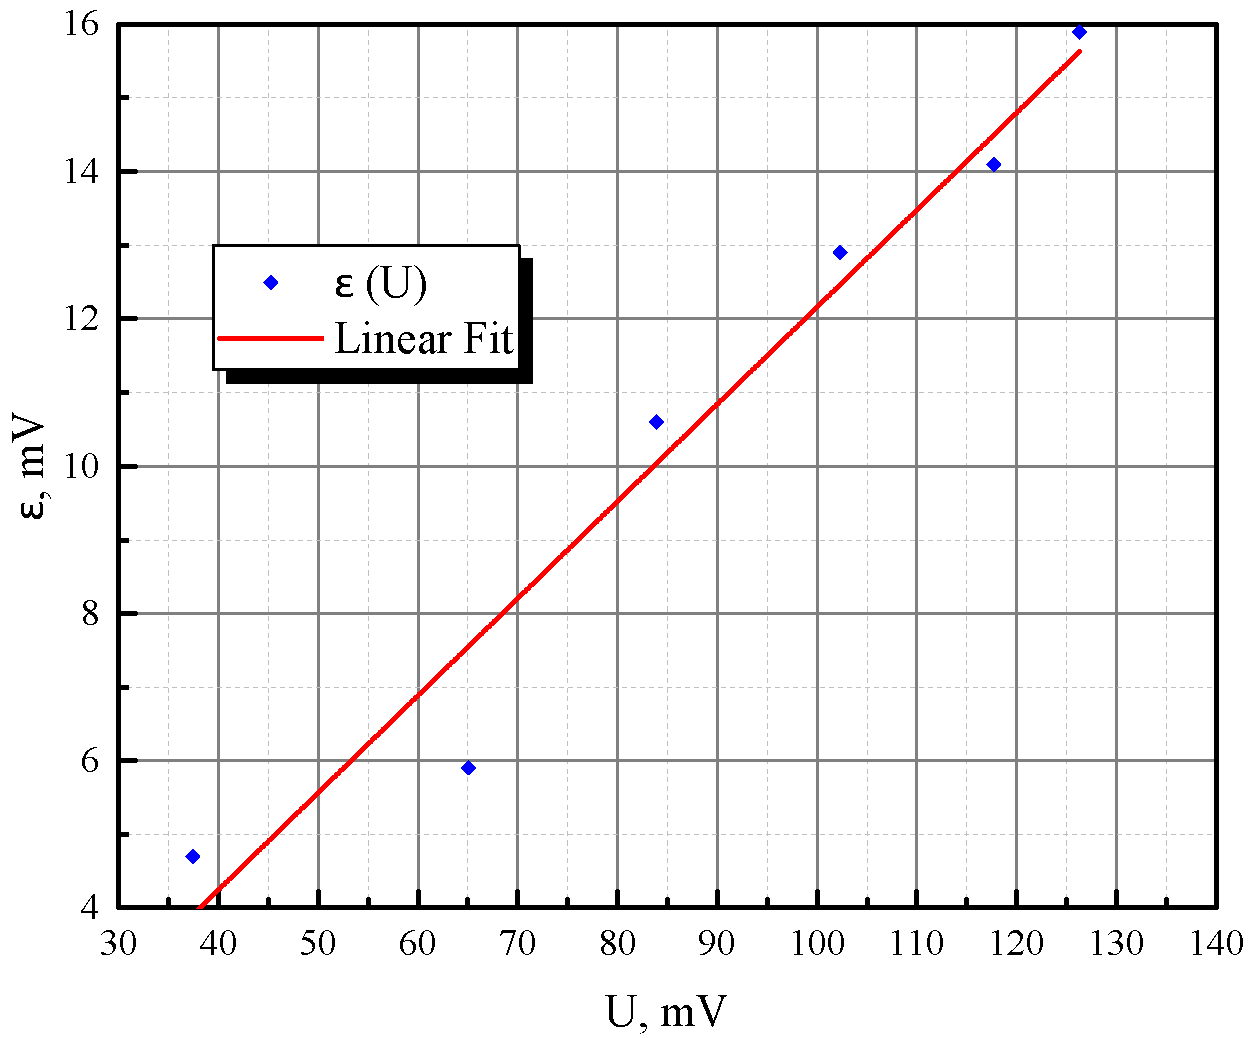
\includegraphics[scale=0.5]{graph.pdf}}
		\caption{Зависимости $U/U_0$ от $\nu/\nu_0$ при различных $R$.}
		\label{ris:graph}
	\end{figure}


\thisfloatsetup{floatrowsep=mysep}	
\begin{figure}[h!]
	\begin{floatrow}
		\ffigbox[\FBwidth]{\caption{Пики колебаний при $R = 100$ Ом.}\label{fig::graph_1}}%
		{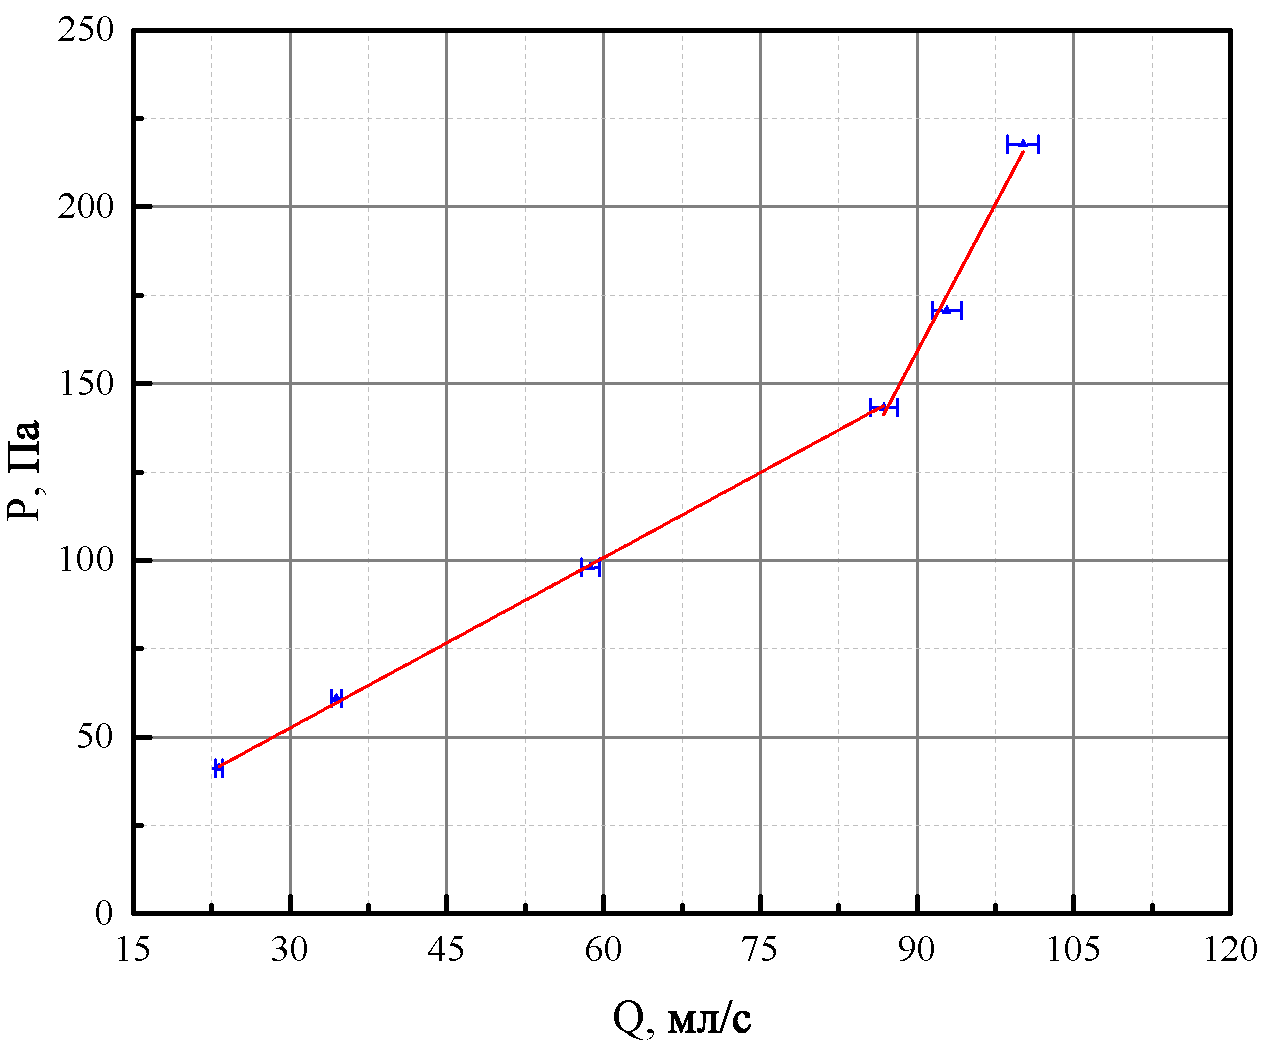
\includegraphics[width=8cm,height=7cm]{Graph_1}}
		\ffigbox[\FBwidth]{\caption{Пики колебаний при $R = 0$ Ом.}\label{fig:graph_2}}%
		{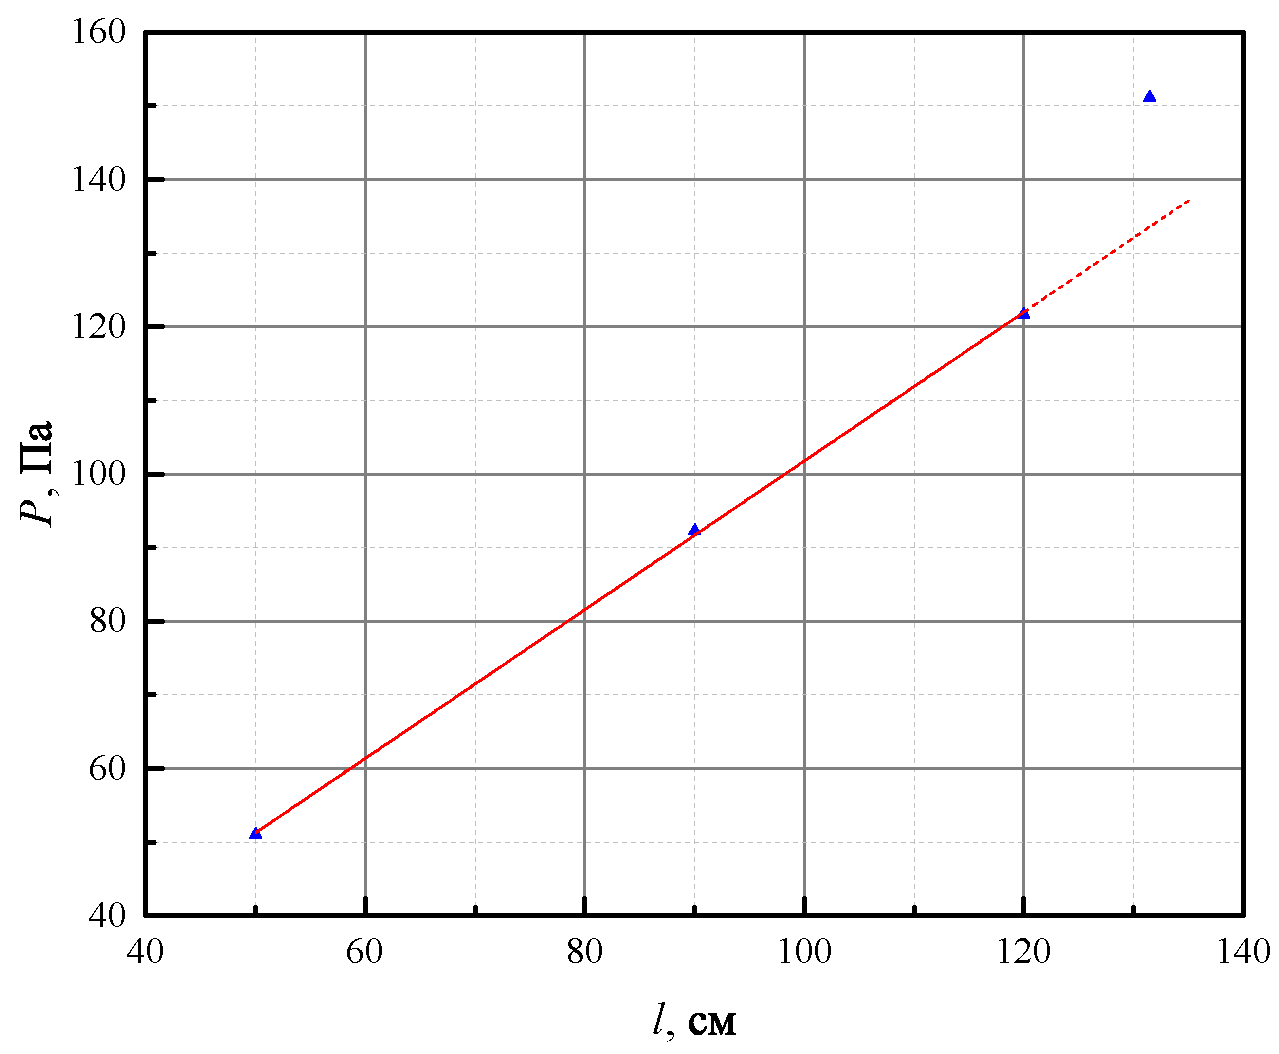
\includegraphics[width=8cm,height=7cm]{Graph_2}}         
	\end{floatrow}
\end{figure}


\section{Выводы}
	Таким образом, мы вычислили добротность контура при различных сопротивлениях резистора рахличными способами $Q = 39,1 \, \pm \, 0,8$ при $R = 0$ Ом и $Q = 7,96 \, \pm \, 0,16$ при $R = 100$ Ом. Результаты вычислений различными способами в пределах погрешностей совпадают.
	
	
\end{document}